\subsection{DiauproPlugin}

The DiauproPlugin is the plugin that runs in the host DAW application. It passes audio data from the host DAW application to three internal processors in series. The first processor is a "Null Process Block" that does no actual audio processing but is usefull for gathering data regarding timing. The second processor is the VCO block that generates a tone based on recieved midi data. The third block is the VCA that shapes the amplitude of the tone over time.

\begin{figure}[H]
    \centering
    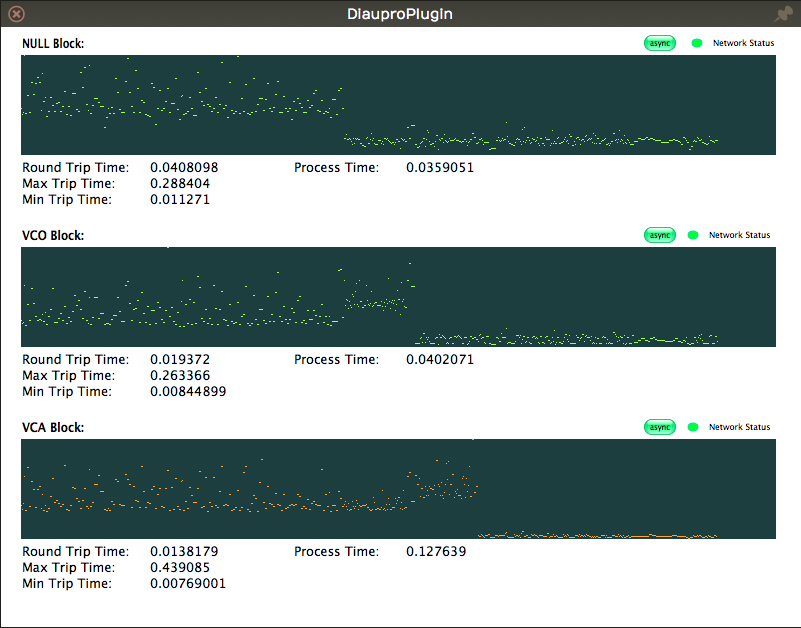
\includegraphics[width=\textwidth]{assets/plugin.png}
    \caption{Screenshot of Plugin GUI}
    \label{fig:plugin}
\end{figure}

The audio plugin's user interface provides feedback to the user regarding the time and operation of the internal processors. Each processor can perform the calculations locally on the CPU or send it's data to a networked node to be processed. A "Network Status" indicator shows if a networked node is performing the processing. The total time that a processor requires to perform it's operations is displayed as the "Round Trip Time". The "Process Time" displays the amount of time that a remote SBC required to perform the processing.

A button is provided that allows the user to switch to an asynchronous processing method. When this is activated each process checks for the availability of the SBC's response, but if it is not yet available is does not wait. Instead the process simply returns empty data back to the plugin. By the time the next buffer is requested by the DAW application the first response is available and the processor can immediately return it without waiting. This method creates a delay in the signal of one buffer cycle, but has the advantage the it does not block the CPU while waiting. The delay can usually be compensated for in the DAW application.

In addition to providing a graphical user interface the plugin also saves timing data to a text file.